\FloatBarrier
\subsection{Euclidean distances analysis for Zernike modes PSFs}

	\subsubsection{Preprocessing}
		
		\begin{itemize}
			\item The PSF electric fields matrices are flattened to compute the euclidean distances between 1d vectors.
			\item 70000 datapoint pairs for each zernike datasets are randomly defined. The euclidean distances will be calculated for these selected pairs.
			\item In this case, LP coefficients are also analysed.
		\end{itemize}
			
	\subsubsection{Euclidean distances comparison per number of zernike modes}
	
		\begin{figure*}[ht!]
			\centering
			\subfloat[Euclidean distance comparison between coefficients and PL flux]{%
				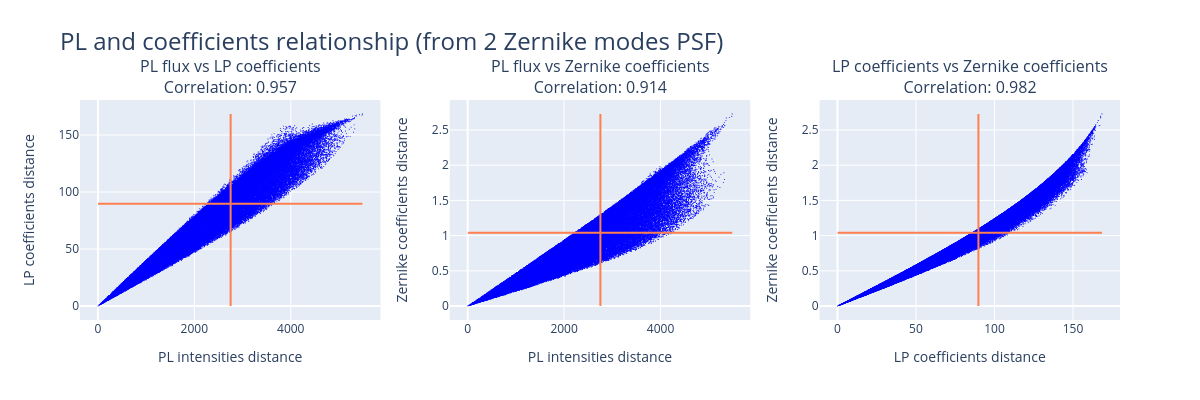
\includegraphics[width=0.7\textwidth]{pid-2mcoefficientsdistances.png}}
			\\
			\subfloat[Euclidean distances for PSF intensity]{%
				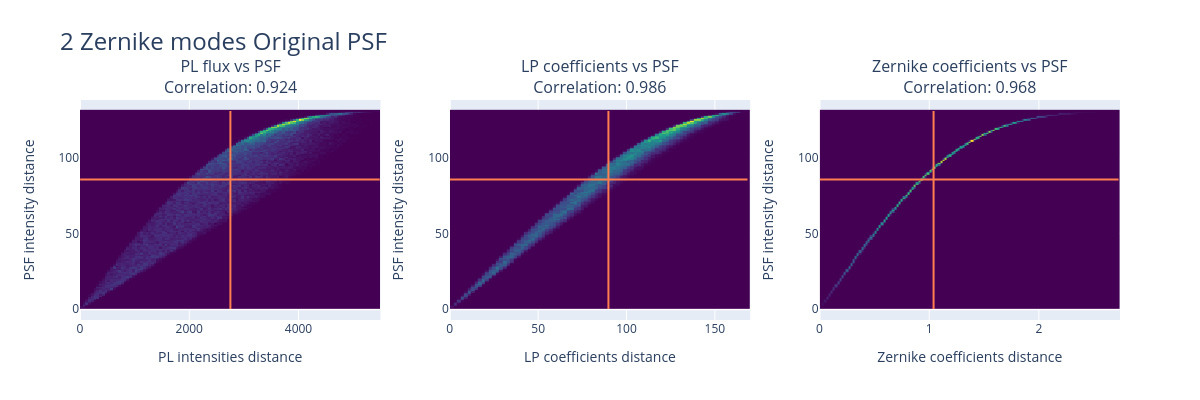
\includegraphics[width=0.7\textwidth]{pid-2mOriginalpsfdistances.png}}
			\\
			\subfloat[Euclidean distances for predicted PSF intensity]{%
				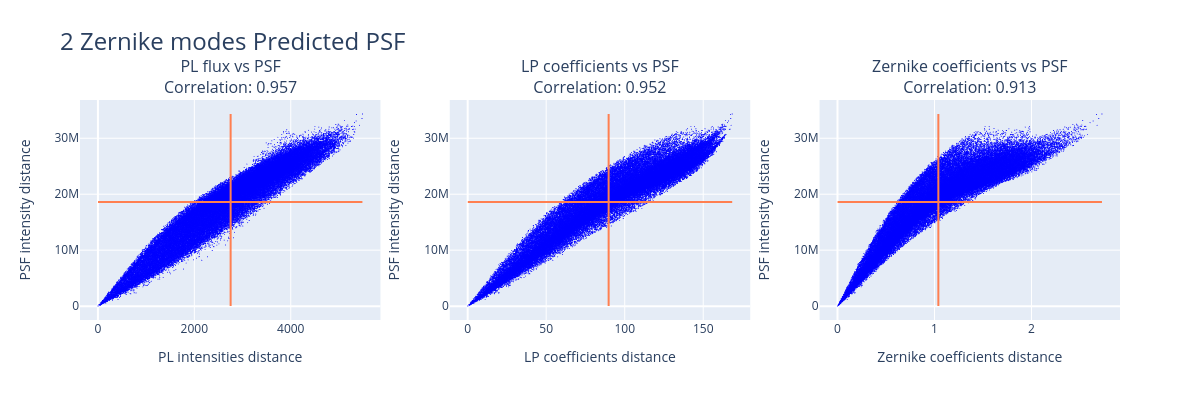
\includegraphics[width=0.7\textwidth]{pid-2mPredictedpsfdistances.png}}
			\\
			\subfloat[Euclidean distances for cropped PSF intensity]{%
				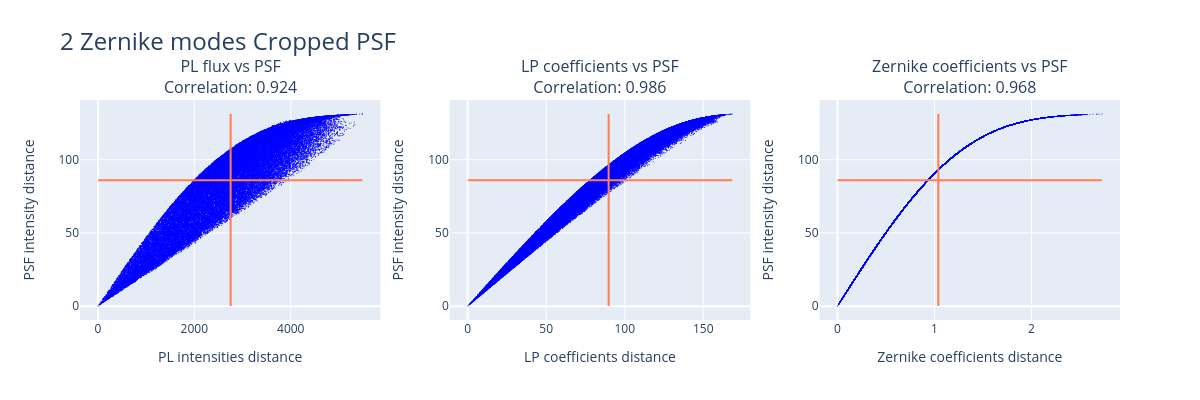
\includegraphics[width=0.7\textwidth]{pid-2mCroppedpsfdistances.png}}
			\\
			\subfloat[Euclidean distances for predicted PSF intensity]{%
				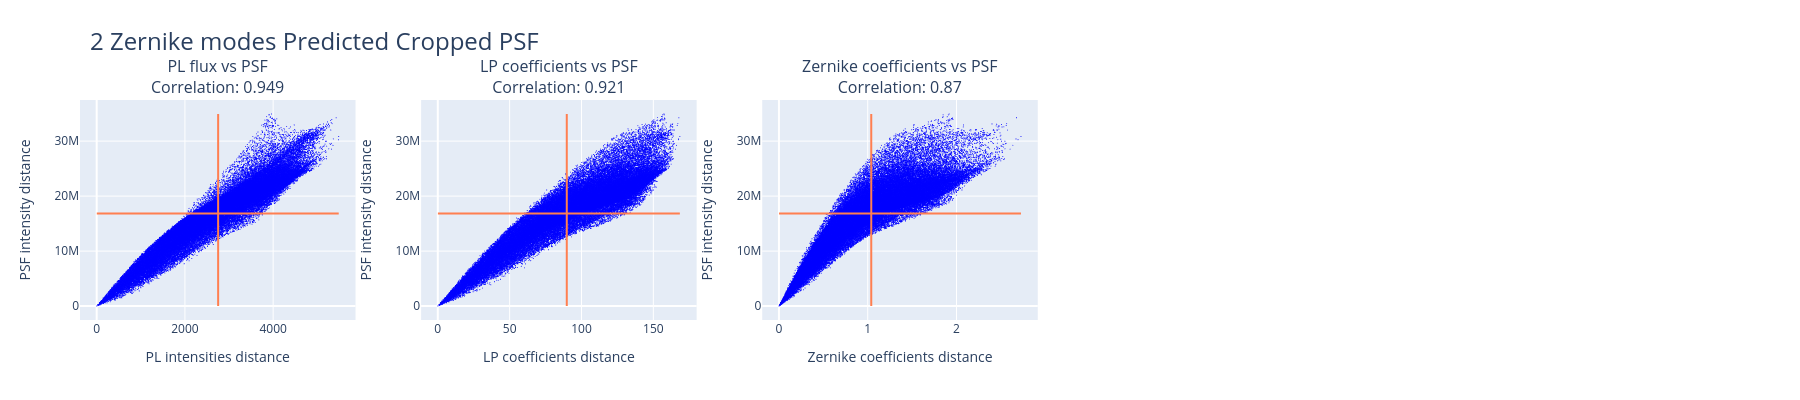
\includegraphics[width=0.7\textwidth]{pid-2mPredicted Croppedpsfdistances.png}}
				
			\caption{Euclidean distances comparison for 2 zernike modes related datasets}
		\end{figure*}
		\FloatBarrier
		
		\begin{figure*}[ht!]
			\centering
			\subfloat[Euclidean distance comparison between coefficients and PL flux]{%
				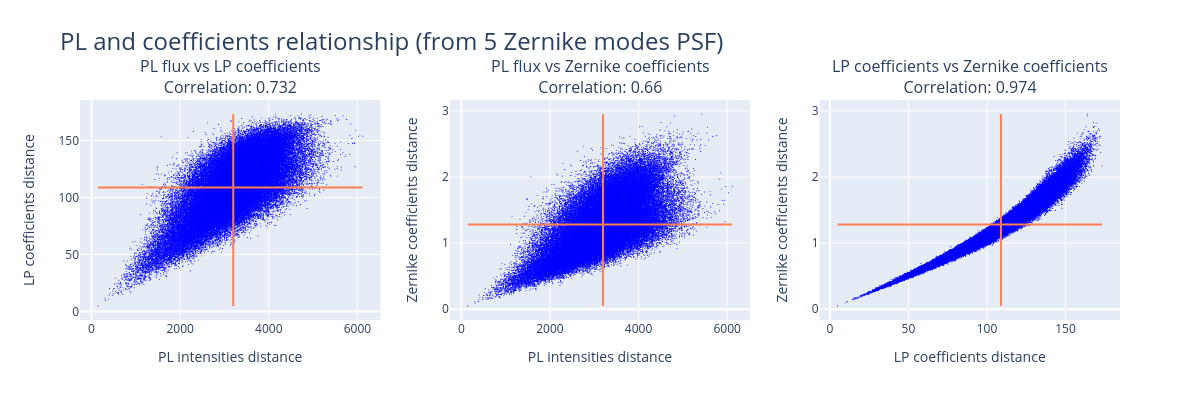
\includegraphics[width=0.7\textwidth]{pid-5mcoefficientsdistances.png}}
			\\
			\subfloat[Euclidean distances for PSF intensity]{%
				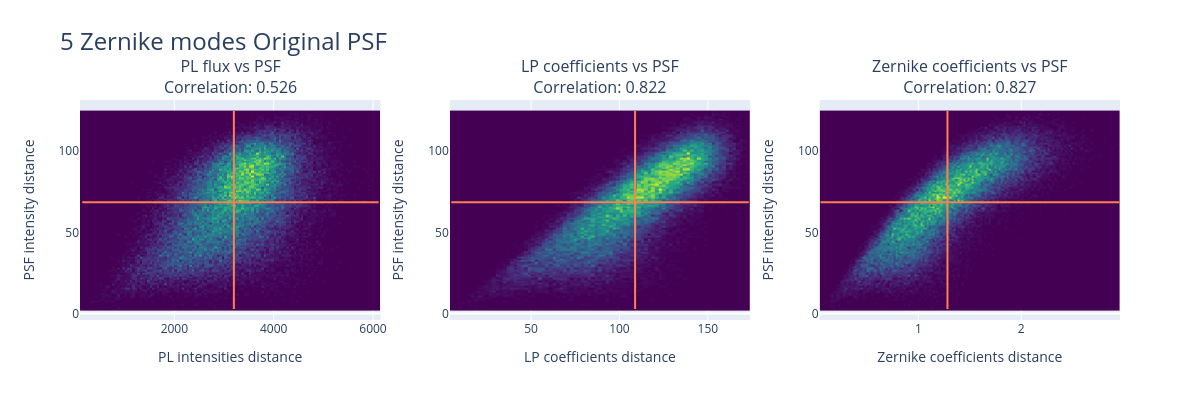
\includegraphics[width=0.7\textwidth]{pid-5mOriginalpsfdistances.png}}
			\\
			\subfloat[Euclidean distances for predicted PSF intensity]{%
				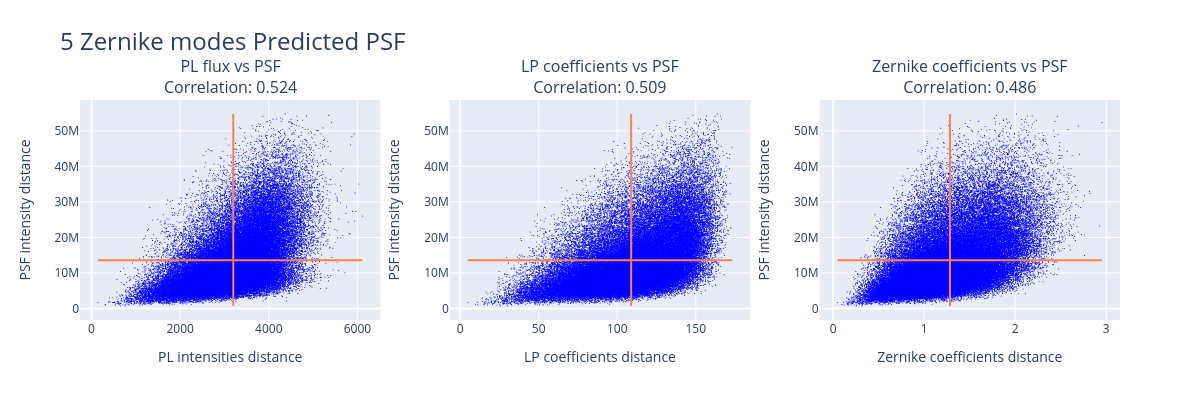
\includegraphics[width=0.7\textwidth]{pid-5mPredictedpsfdistances.png}}
			\\
			\subfloat[Euclidean distances for cropped PSF intensity]{%
				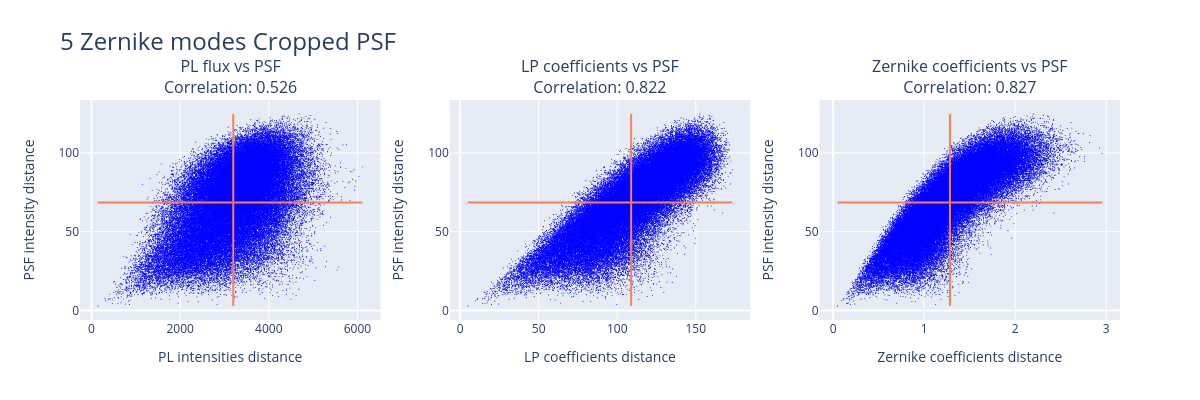
\includegraphics[width=0.7\textwidth]{pid-5mCroppedpsfdistances.png}}
			\\
			\subfloat[Euclidean distances for predicted PSF intensity]{%
				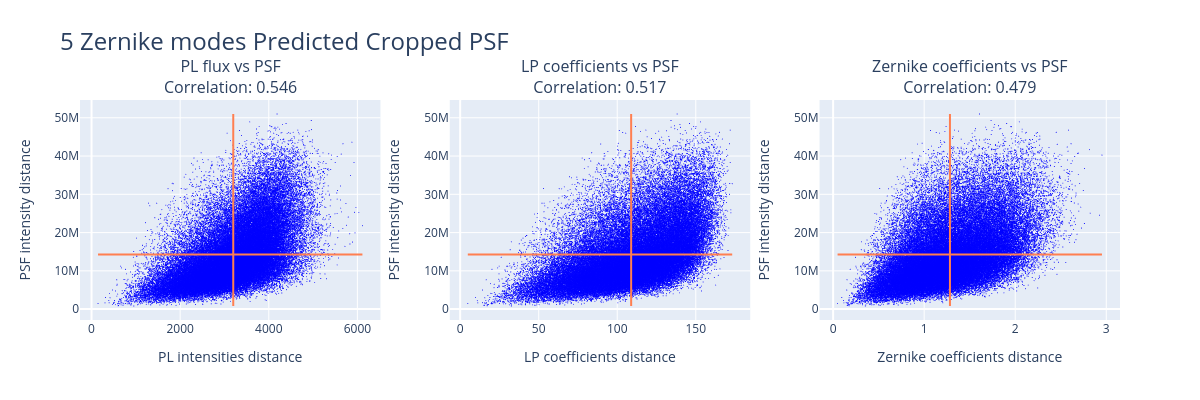
\includegraphics[width=0.7\textwidth]{pid-5mPredicted Croppedpsfdistances.png}}
				
			\caption{Euclidean distances comparison for 5 zernike modes related datasets}
		\end{figure*}
		\FloatBarrier
		
		\begin{figure*}[ht!]
			\centering
			\subfloat[Euclidean distance comparison between coefficients and PL flux]{%
				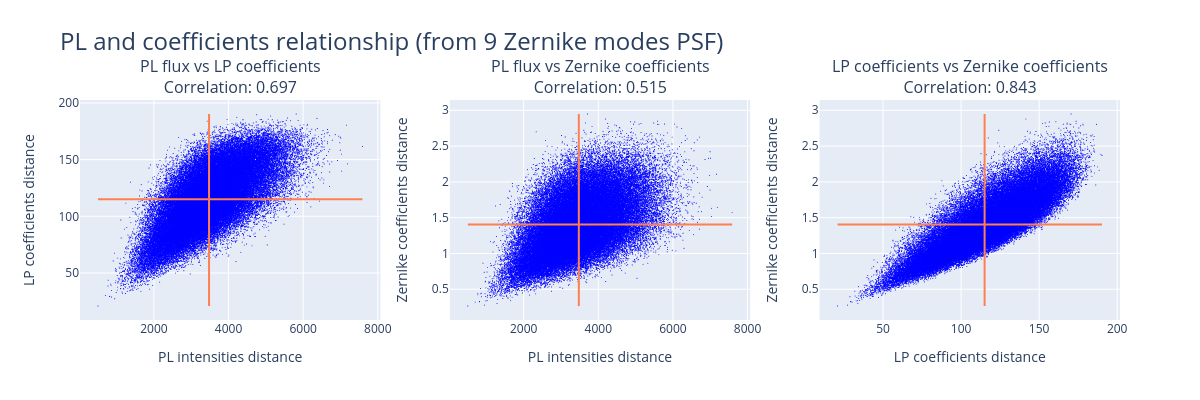
\includegraphics[width=0.7\textwidth]{pid-9mcoefficientsdistances.png}}
			\\
			\subfloat[Euclidean distances for PSF intensity]{%
				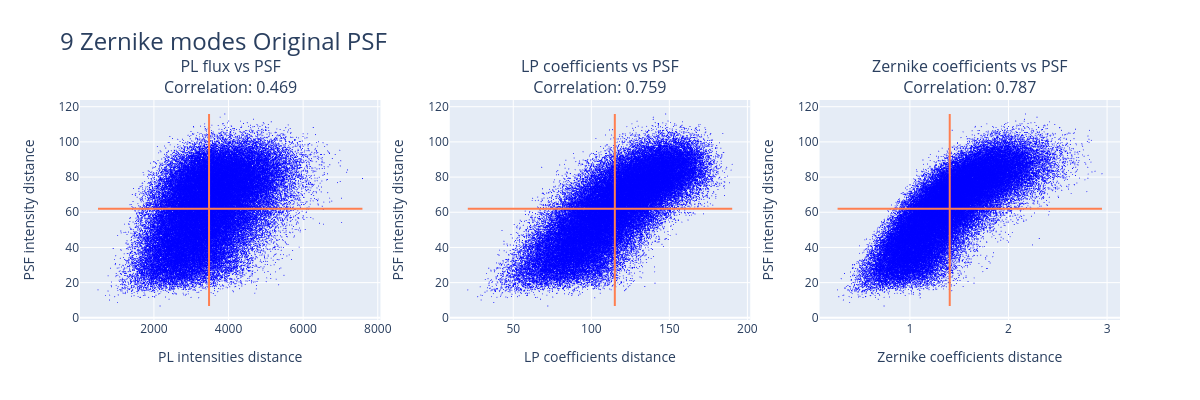
\includegraphics[width=0.7\textwidth]{pid-9mOriginalpsfdistances.png}}
			\\
			\subfloat[Euclidean distances for predicted PSF intensity]{%
				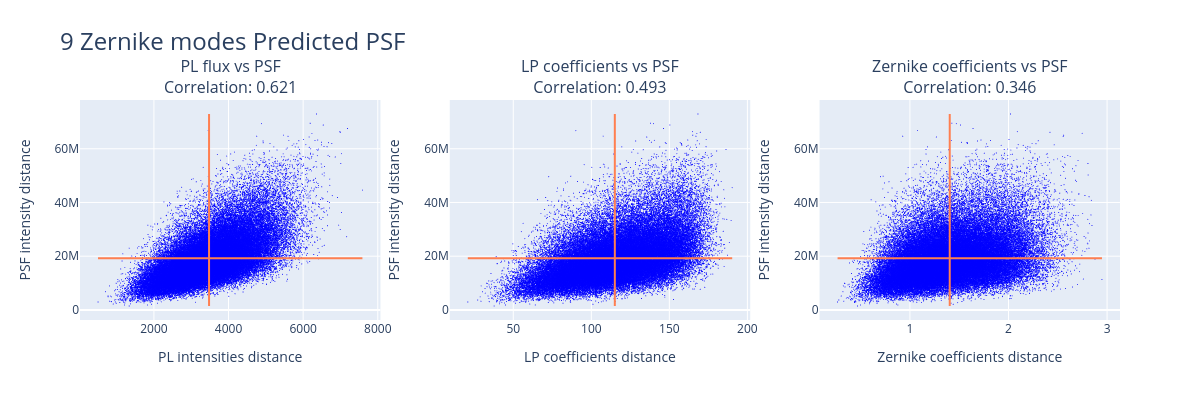
\includegraphics[width=0.7\textwidth]{pid-9mPredictedpsfdistances.png}}
			\\
			\subfloat[Euclidean distances for cropped PSF intensity]{%
				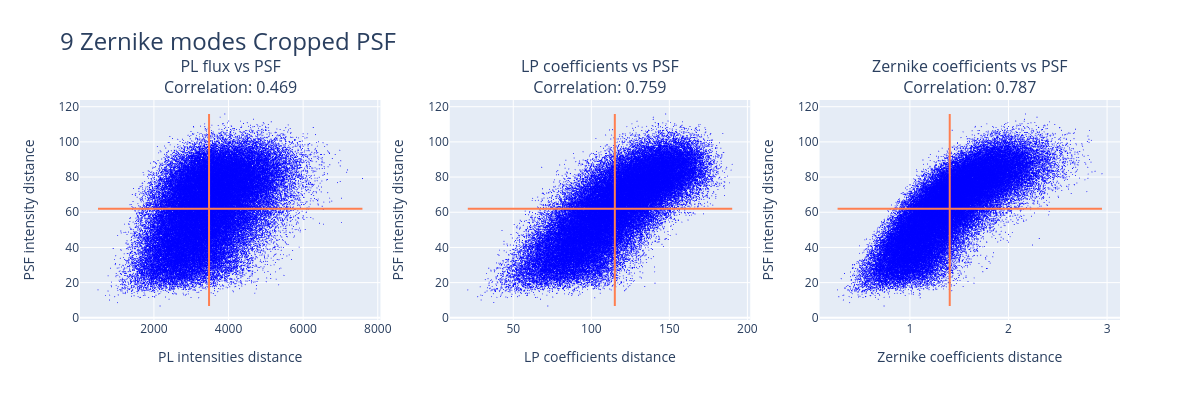
\includegraphics[width=0.7\textwidth]{pid-9mCroppedpsfdistances.png}}
			\\
			\subfloat[Euclidean distances for predicted PSF intensity]{%
				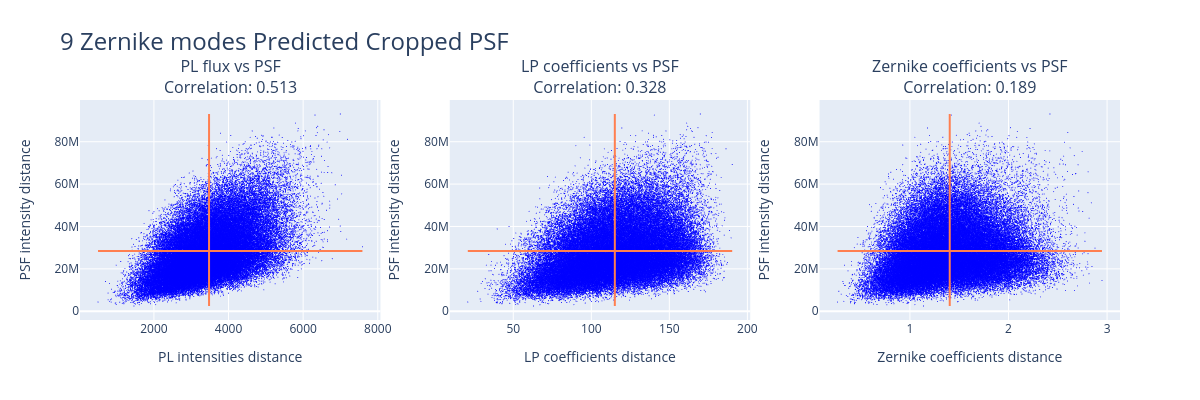
\includegraphics[width=0.7\textwidth]{pid-9mPredicted Croppedpsfdistances.png}}
				
			\caption{Euclidean distances comparison for 9 zernike modes related datasets}
		\end{figure*}
		\FloatBarrier
		
		\begin{figure*}[ht!]
			\centering
			\subfloat[Euclidean distance comparison between coefficients and PL flux]{%
				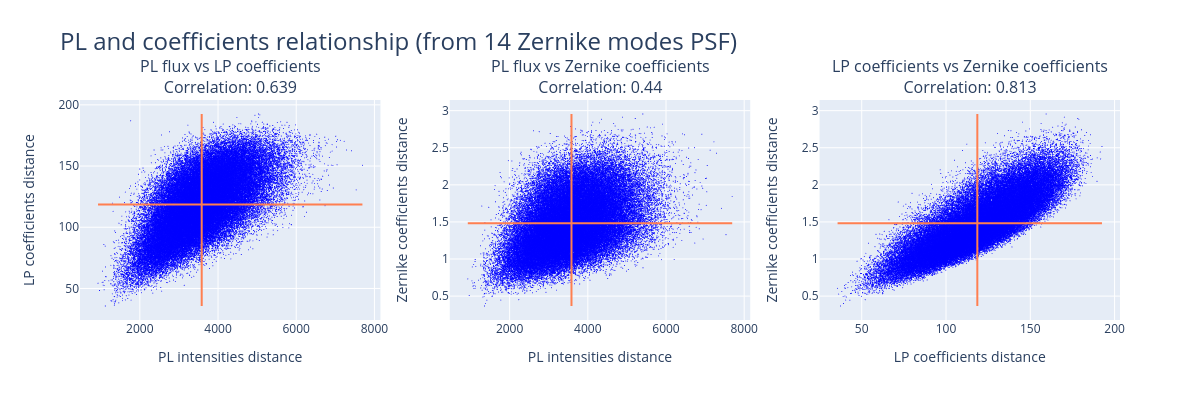
\includegraphics[width=0.7\textwidth]{pid-14mcoefficientsdistances.png}}
			\\
			\subfloat[Euclidean distances for PSF intensity]{%
				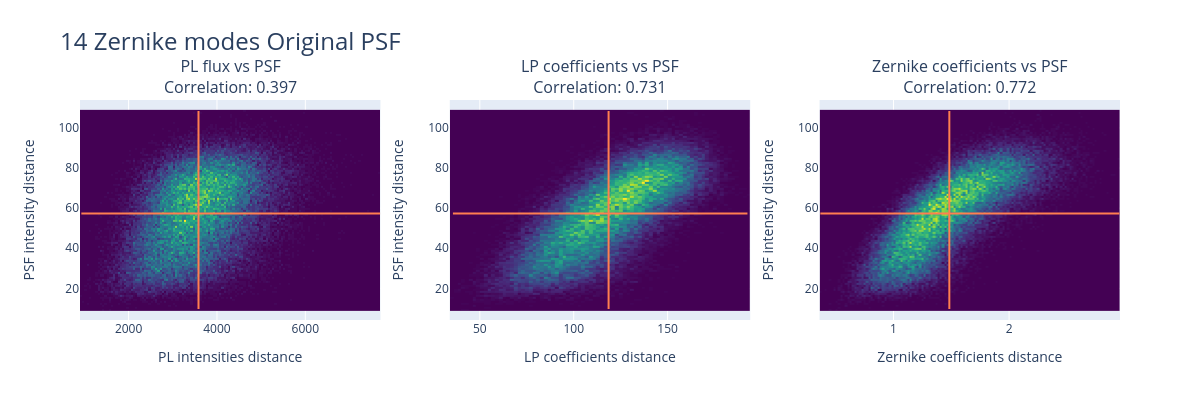
\includegraphics[width=0.7\textwidth]{pid-14mOriginalpsfdistances.png}}
			\\
			\subfloat[Euclidean distances for predicted PSF intensity]{%
				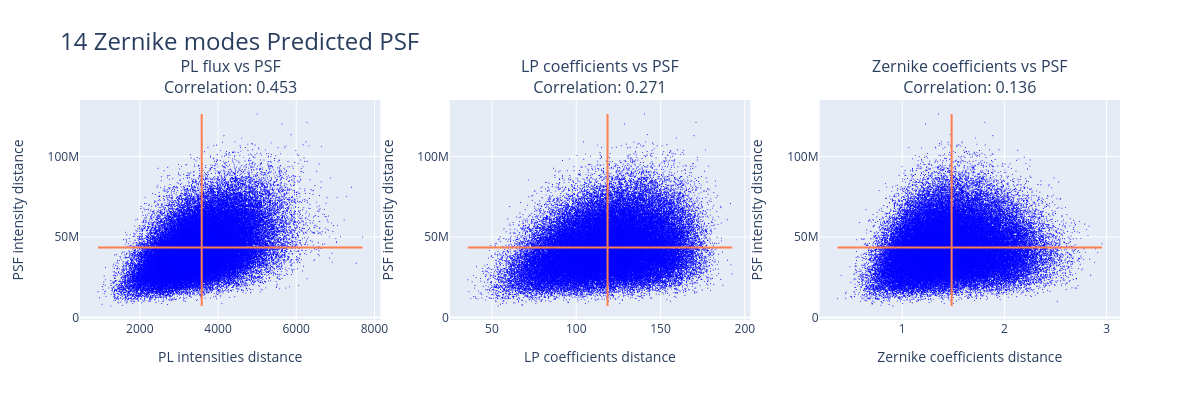
\includegraphics[width=0.7\textwidth]{pid-14mPredictedpsfdistances.png}}
			\\
			\subfloat[Euclidean distances for cropped PSF intensity]{%
				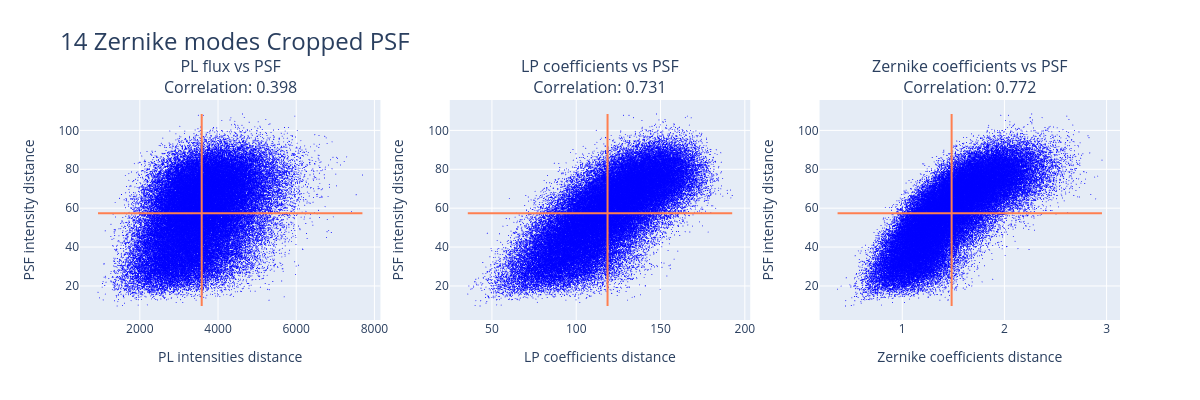
\includegraphics[width=0.7\textwidth]{pid-14mCroppedpsfdistances.png}}
			\\
			\subfloat[Euclidean distances for predicted PSF intensity]{%
				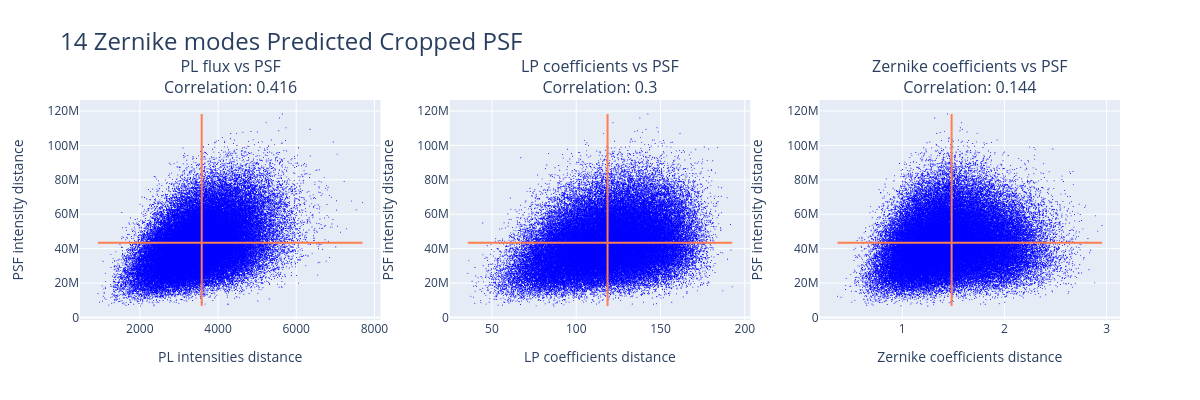
\includegraphics[width=0.7\textwidth]{pid-14mPredicted Croppedpsfdistances.png}}
				
			\caption{Euclidean distances comparison for 14 zernike modes related datasets}
		\end{figure*}
		\FloatBarrier
		
		\begin{figure*}[ht!]
			\centering
			\subfloat[Euclidean distance comparison between coefficients and PL flux]{%
				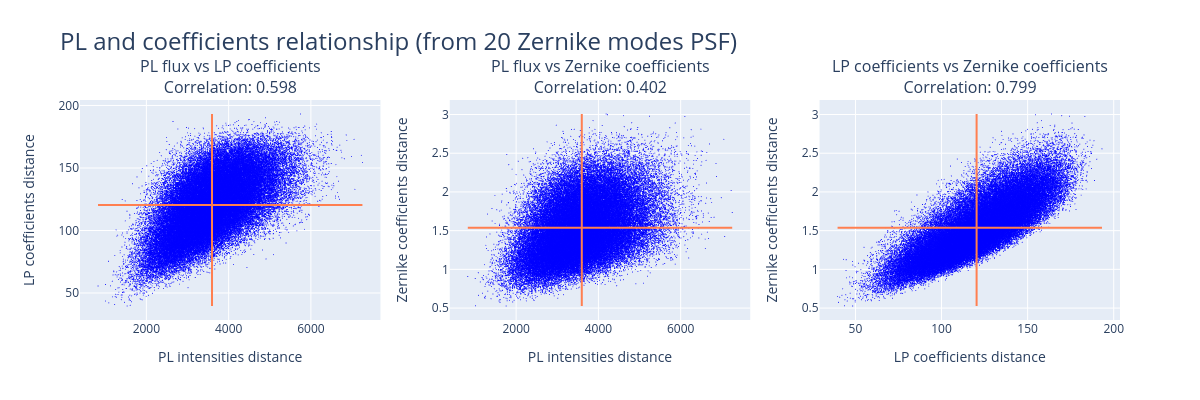
\includegraphics[width=0.7\textwidth]{pid-20mcoefficientsdistances.png}}
			\\
			\subfloat[Euclidean distances for PSF intensity]{%
				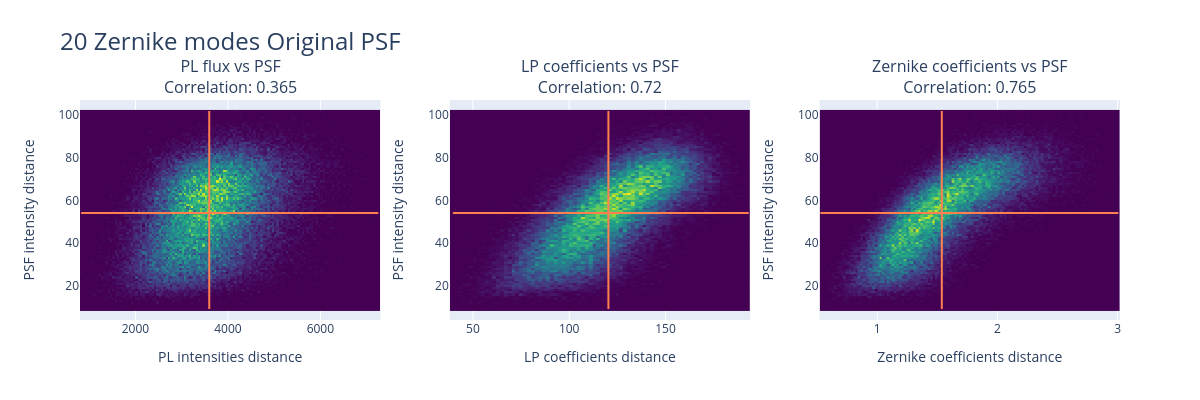
\includegraphics[width=0.7\textwidth]{pid-20mOriginalpsfdistances.png}}
			\\
			\subfloat[Euclidean distances for predicted PSF intensity]{%
				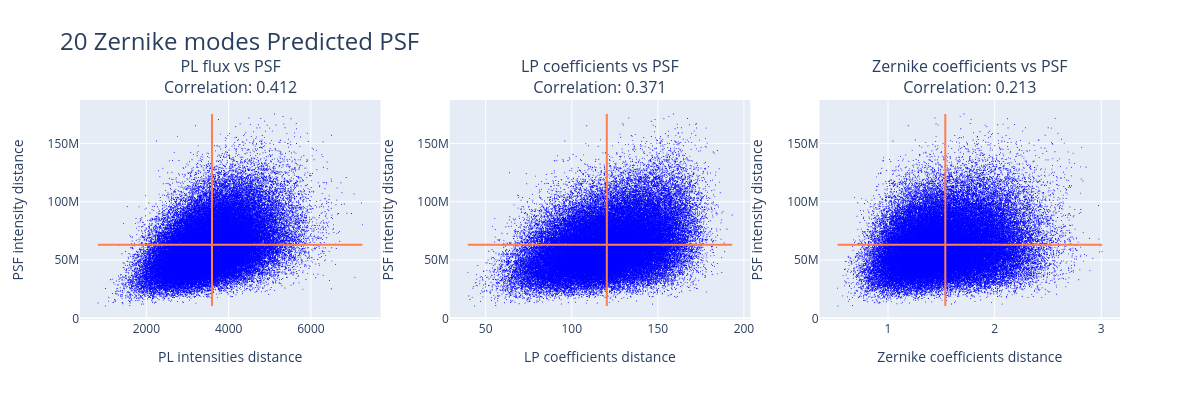
\includegraphics[width=0.7\textwidth]{pid-20mPredictedpsfdistances.png}}
			\\
			\subfloat[Euclidean distances for cropped PSF intensity]{%
				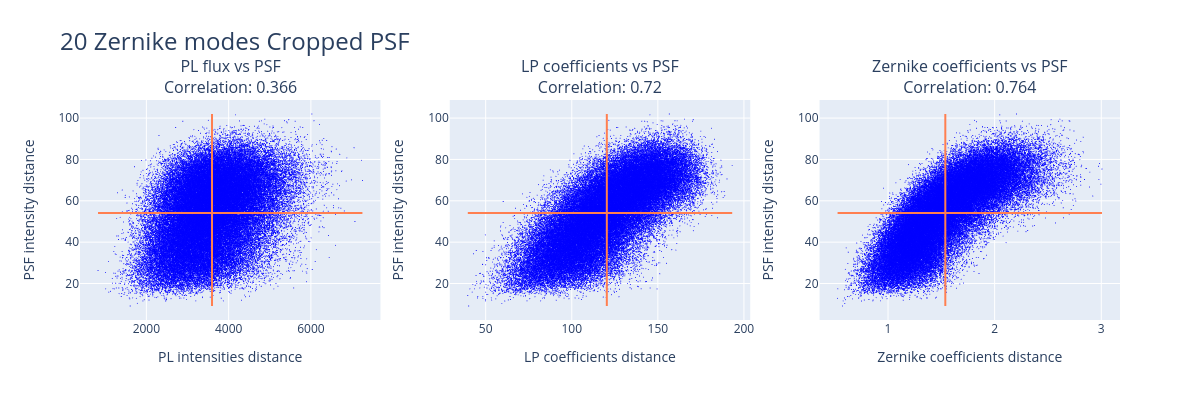
\includegraphics[width=0.7\textwidth]{pid-20mCroppedpsfdistances.png}}
			\\
			\subfloat[Euclidean distances for predicted PSF intensity]{%
				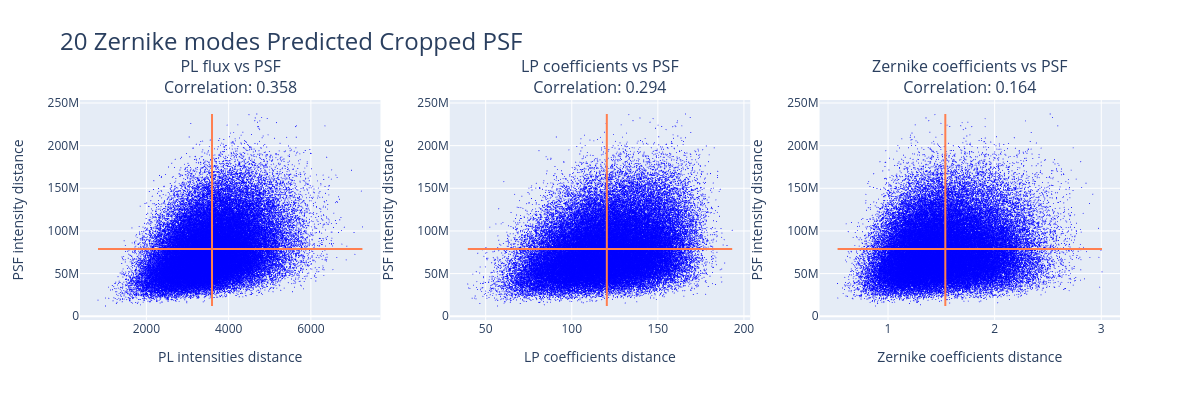
\includegraphics[width=0.7\textwidth]{pid-20mPredicted Croppedpsfdistances.png}}
				
			\caption{Euclidean distances comparison for 20 zernike modes related datasets}
		\end{figure*}
	
	\FloatBarrier
	\subsubsection{Euclidean distances comparison evolution over number of zernike modes}
	
		\begin{figure*}[ht!]
			\centering
			\subfloat[Coefficients vs PL flux for 2 zernike modes]{%
				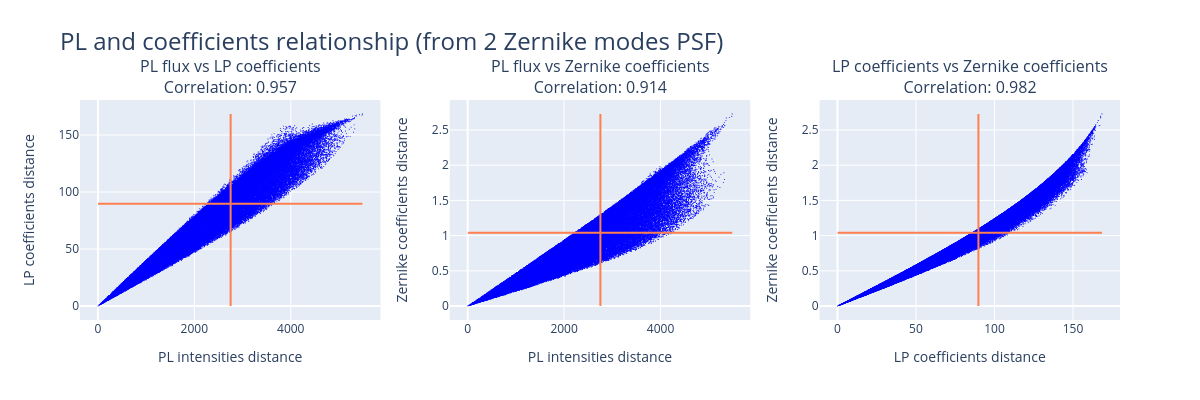
\includegraphics[width=0.7\textwidth]{pid-2mcoefficientsdistances.png}}
			\\
			\subfloat[Coefficients vs PL flux for 5 zernike modes]{%
				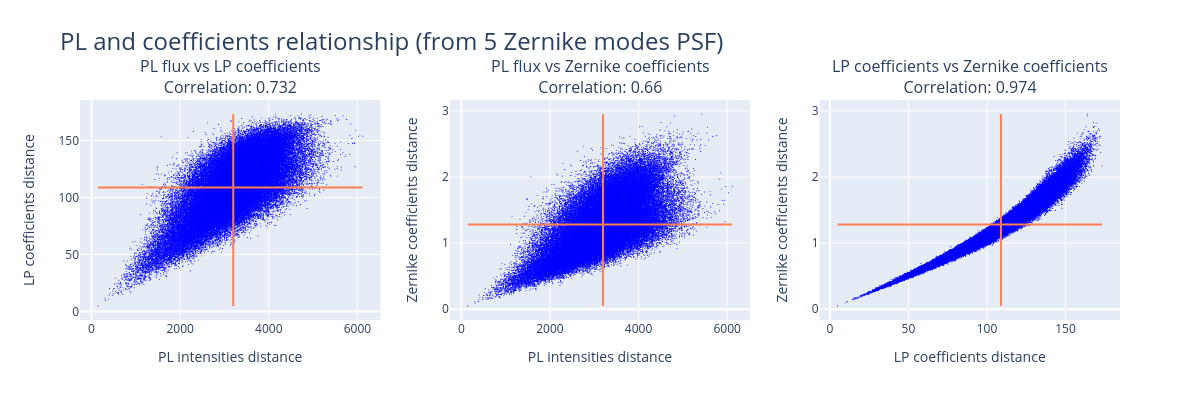
\includegraphics[width=0.7\textwidth]{pid-5mcoefficientsdistances.png}}
			\\
			\subfloat[Coefficients vs PL flux for 9 zernike modes]{%
				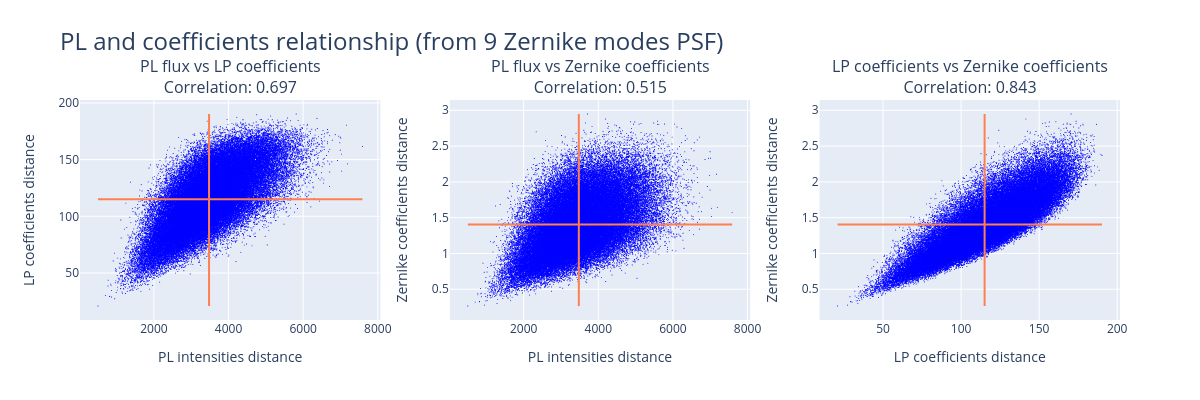
\includegraphics[width=0.7\textwidth]{pid-9mcoefficientsdistances.png}}
			\\
			\subfloat[Coefficients vs PL flux for 14 zernike modes]{%
				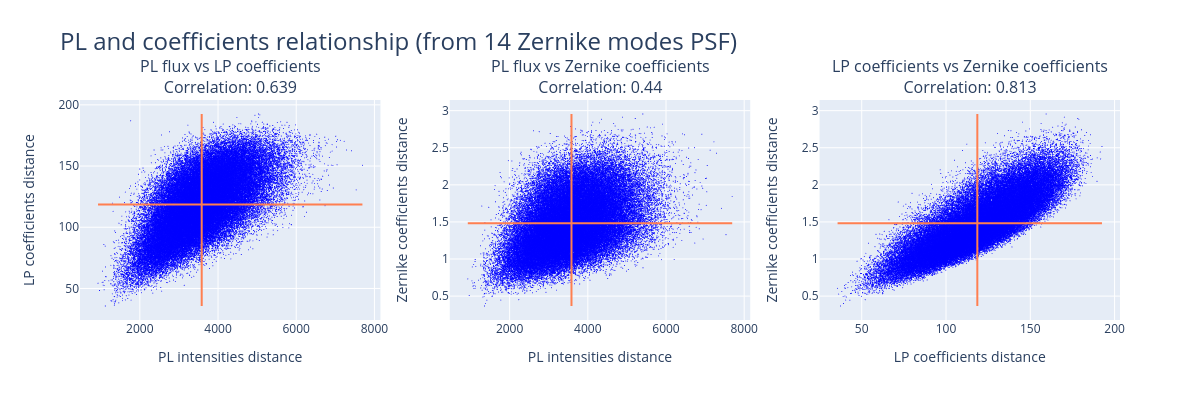
\includegraphics[width=0.7\textwidth]{pid-14mcoefficientsdistances.png}}
			\\
			\subfloat[Coefficients vs PL flux for 20 zernike modes]{%
				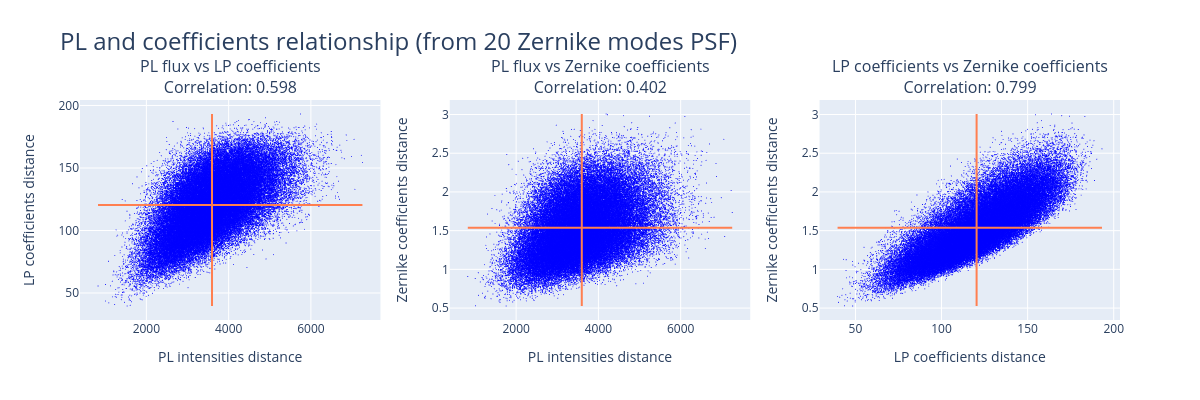
\includegraphics[width=0.7\textwidth]{pid-20mcoefficientsdistances.png}}
				
			\caption{Euclidean distance comparison between coefficients and PL flux for different number of modes}
		\end{figure*}
		\FloatBarrier
		
		
		\begin{figure*}[ht!]
			\centering
			\subfloat[Euclidean distances for 2 zernike modes PSF intensity]{%
				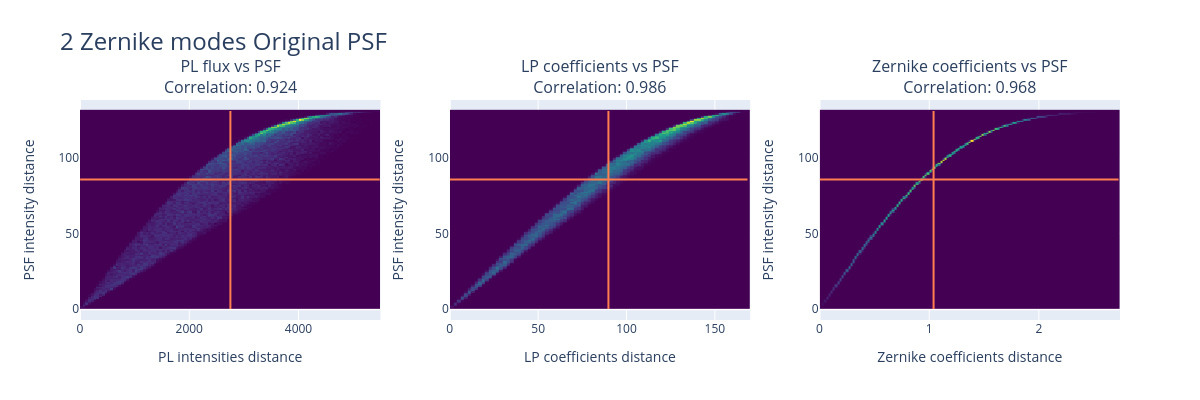
\includegraphics[width=0.7\textwidth]{pid-2mOriginalpsfdistances.png}}
			\\
			\subfloat[Euclidean distances for 5 zernike modes PSF intensity]{%
				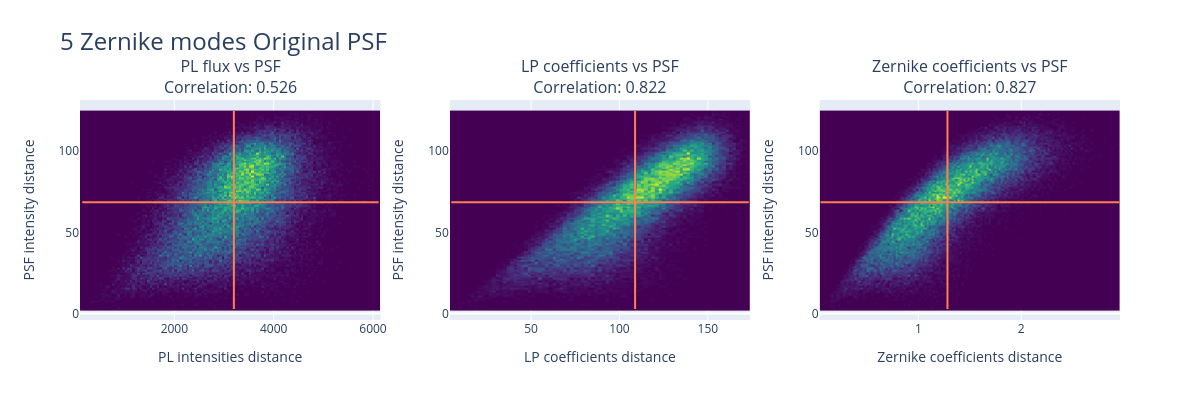
\includegraphics[width=0.7\textwidth]{pid-5mOriginalpsfdistances.png}}
			\\
			\subfloat[Euclidean distances for 9 zernike modes PSF intensity]{%
				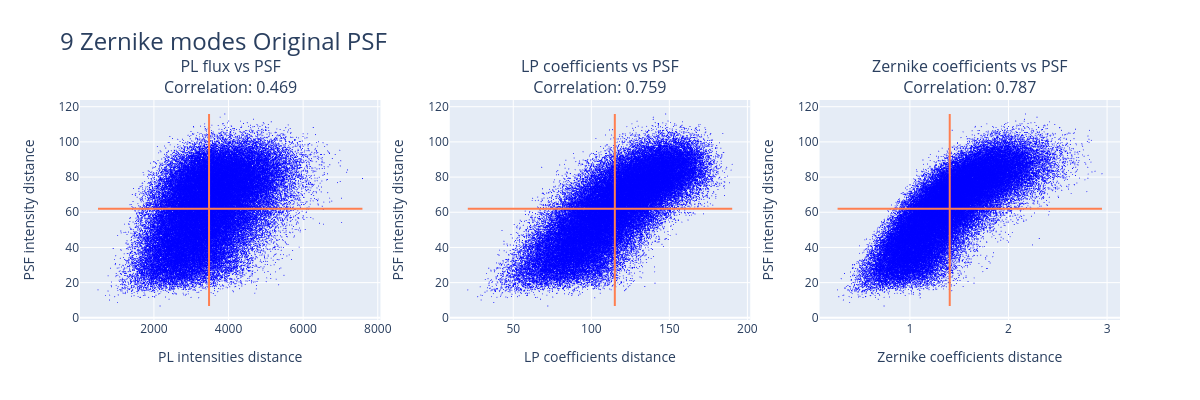
\includegraphics[width=0.7\textwidth]{pid-9mOriginalpsfdistances.png}}
			\\
			\subfloat[Euclidean distances for 14 zernike modes PSF intensity]{%
				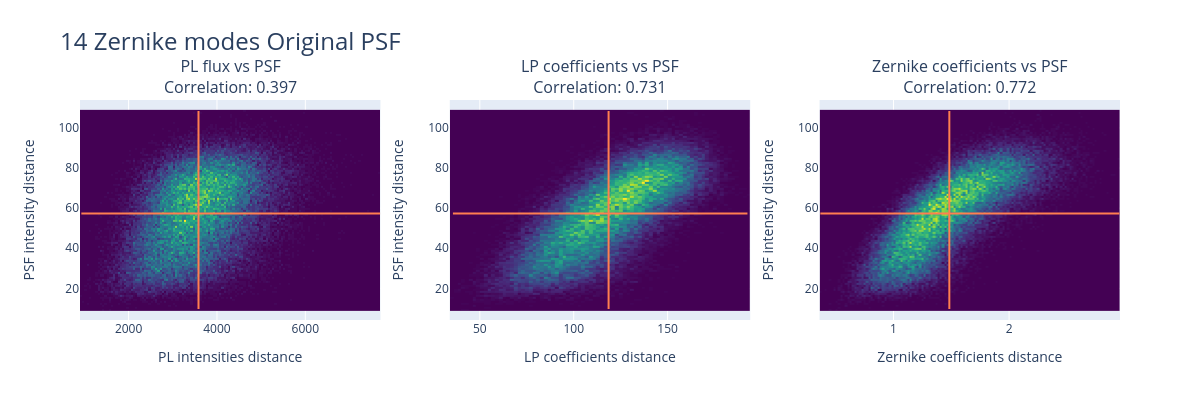
\includegraphics[width=0.7\textwidth]{pid-14mOriginalpsfdistances.png}}
			\\
			\subfloat[Euclidean distances for 20 zernike modes PSF intensity]{%
				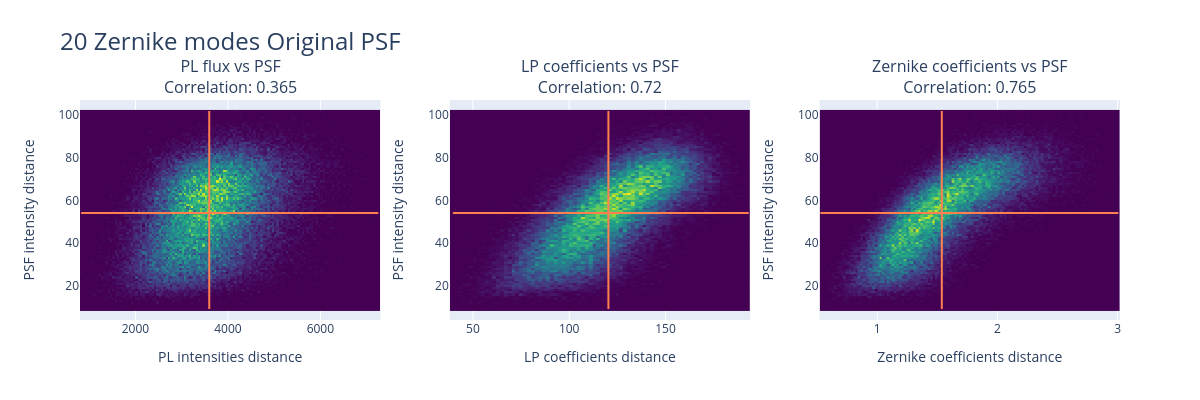
\includegraphics[width=0.7\textwidth]{pid-20mOriginalpsfdistances.png}}
				
			\caption{Euclidean distance comparison for PSF intensity for different number of modes}
		\end{figure*}
		\FloatBarrier
		
		
		\begin{figure*}[ht!]
			\centering
			\subfloat[Euclidean distances for 2 zernike modes predicted PSF intensity]{%
				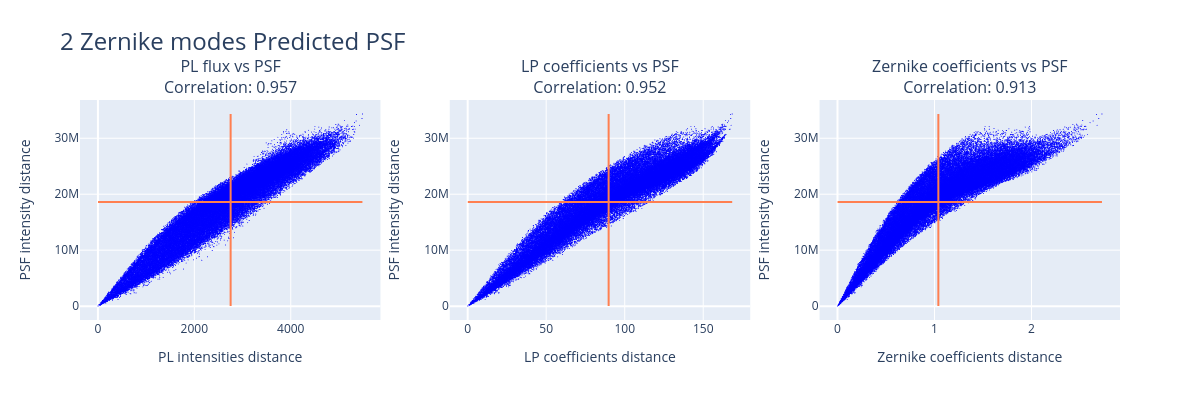
\includegraphics[width=0.7\textwidth]{pid-2mPredictedpsfdistances.png}}
			\\
			\subfloat[Euclidean distances for 5 zernike modes predicted PSF intensity]{%
				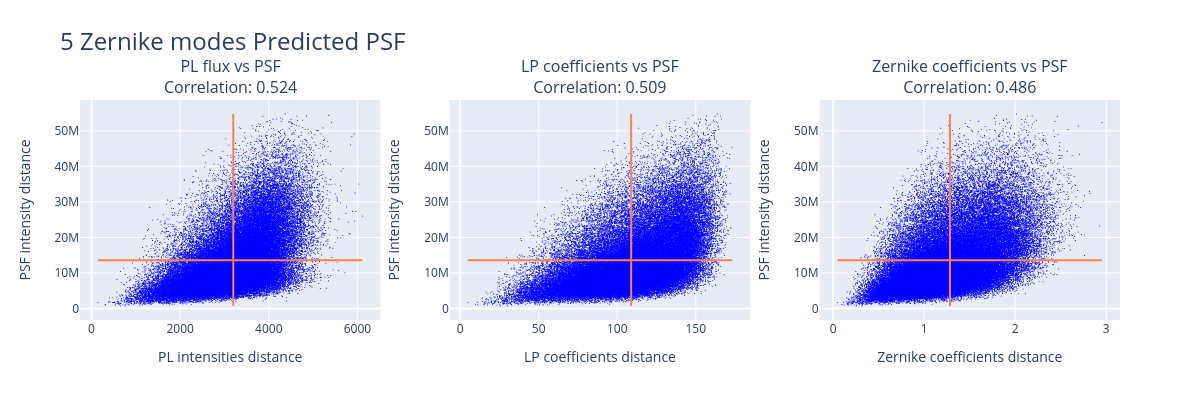
\includegraphics[width=0.7\textwidth]{pid-5mPredictedpsfdistances.png}}
			\\
			\subfloat[Euclidean distances for 9 zernike modes predicted PSF intensity]{%
				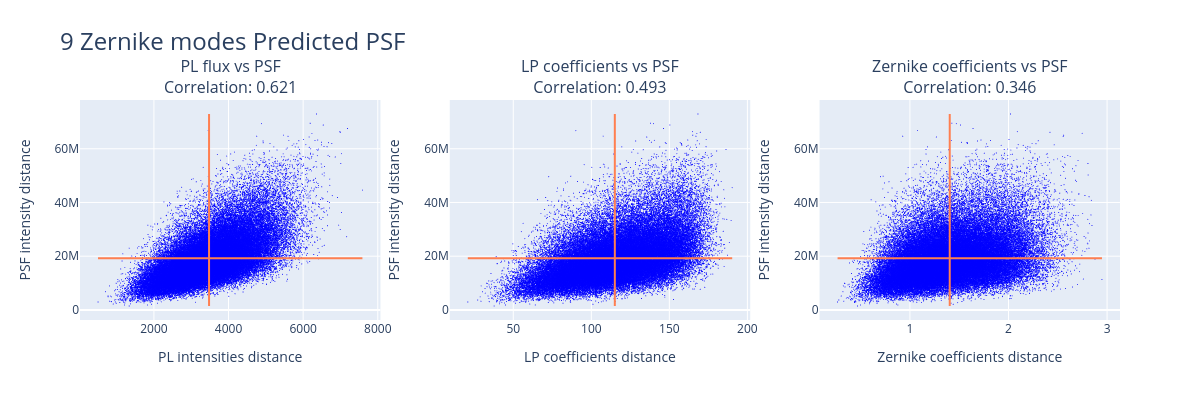
\includegraphics[width=0.7\textwidth]{pid-9mPredictedpsfdistances.png}}
			\\
			\subfloat[Euclidean distances for 14 zernike modes predicted PSF intensity]{%
				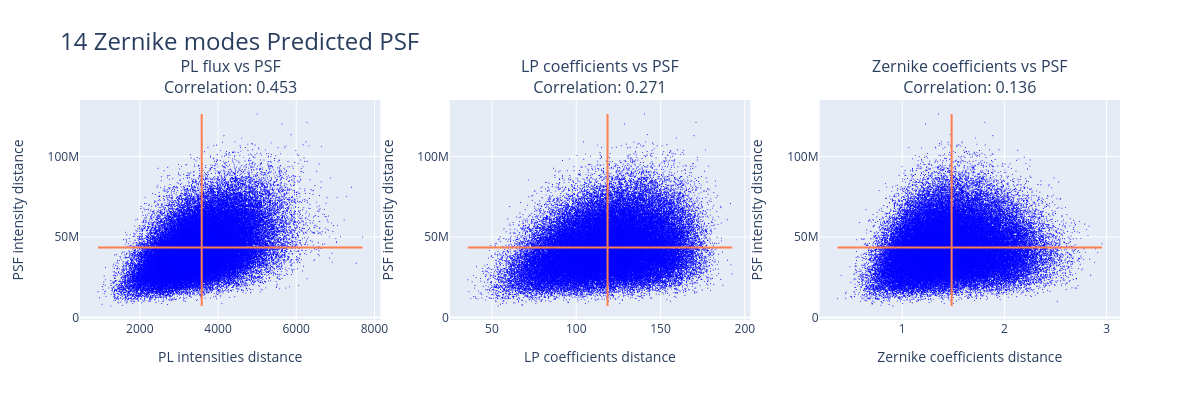
\includegraphics[width=0.7\textwidth]{pid-14mPredictedpsfdistances.png}}
			\\
			\subfloat[Euclidean distances for 20 zernike modes predicted PSF intensity]{%
				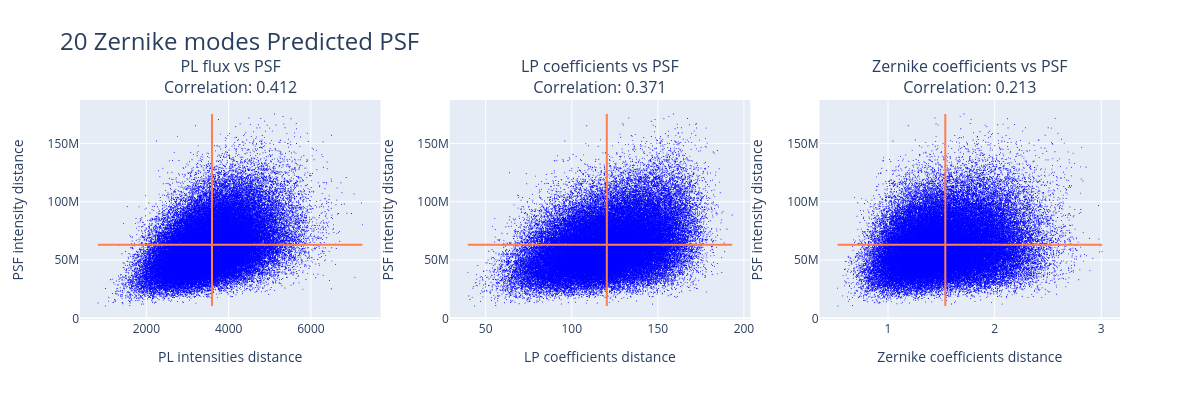
\includegraphics[width=0.7\textwidth]{pid-20mPredictedpsfdistances.png}}
				
			\caption{Euclidean distance comparison for predicted PSF intensity for different number of modes}
		\end{figure*}
		\FloatBarrier
		
		
		\begin{figure*}[ht!]
			\centering
			\subfloat[Euclidean distances for 2 zernike modes cropped PSF intensity]{%
				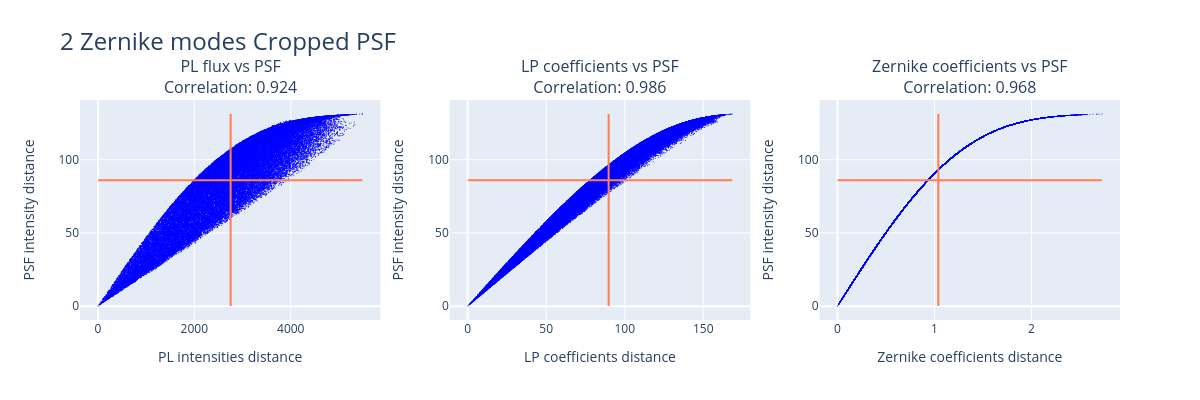
\includegraphics[width=0.7\textwidth]{pid-2mCroppedpsfdistances.png}}
			\\
			\subfloat[Euclidean distances for 5 zernike modes cropped PSF intensity]{%
				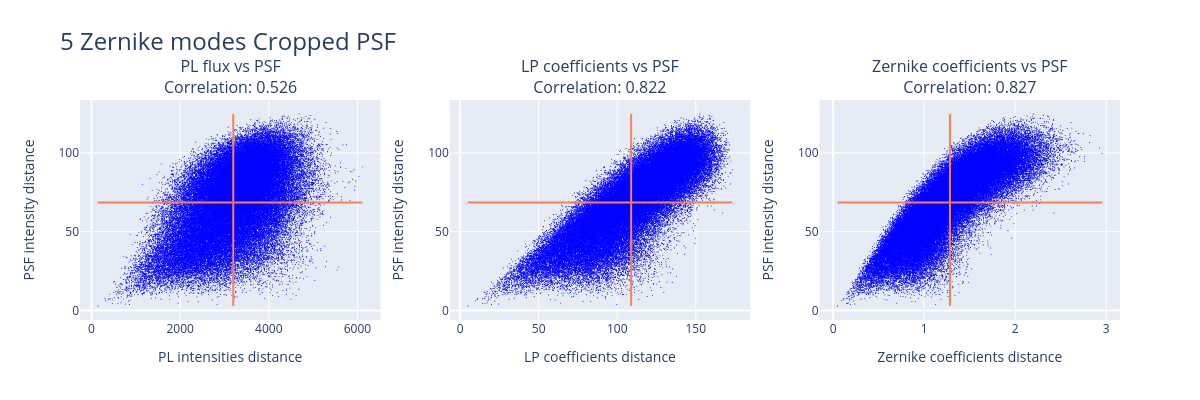
\includegraphics[width=0.7\textwidth]{pid-5mCroppedpsfdistances.png}}
			\\
			\subfloat[Euclidean distances for 9 zernike modes cropped PSF intensity]{%
				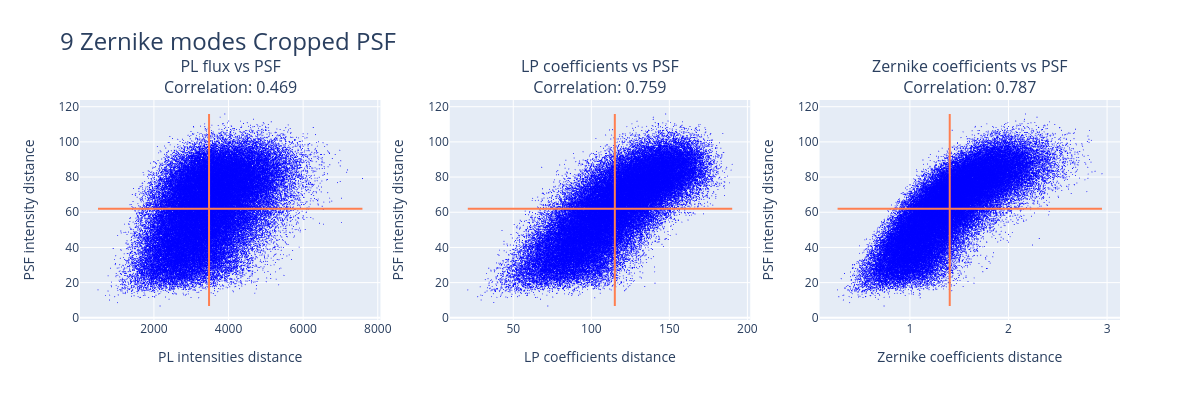
\includegraphics[width=0.7\textwidth]{pid-9mCroppedpsfdistances.png}}
			\\
			\subfloat[Euclidean distances for 14 zernike modes cropped PSF intensity]{%
				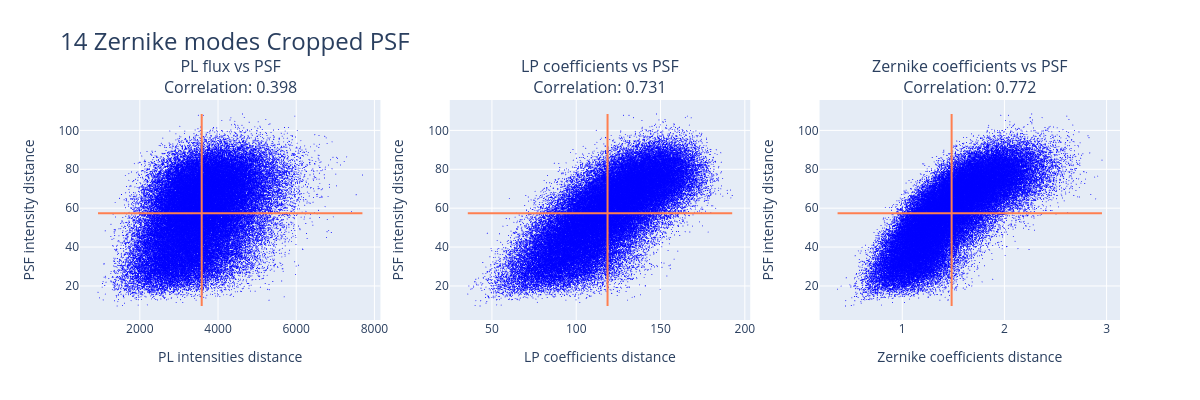
\includegraphics[width=0.7\textwidth]{pid-14mCroppedpsfdistances.png}}
			\\
			\subfloat[Euclidean distances for 20 zernike modes cropped PSF intensity]{%
				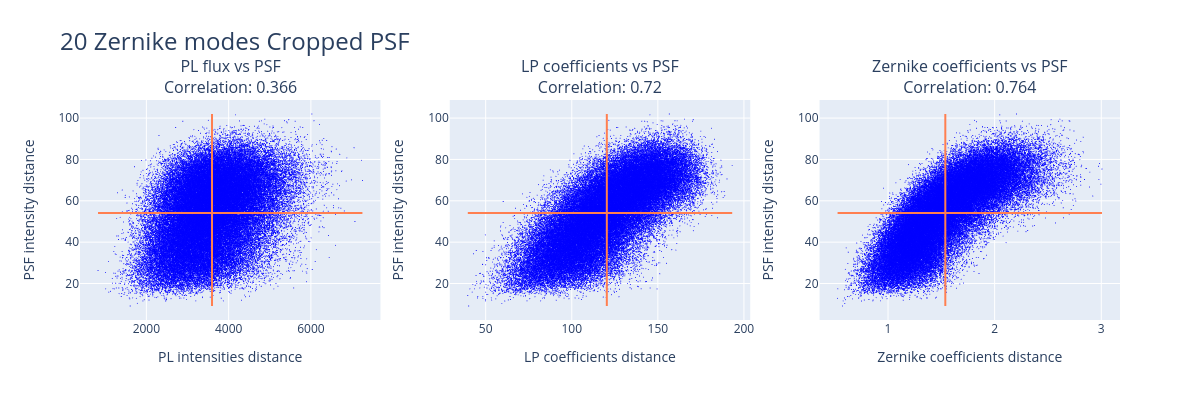
\includegraphics[width=0.7\textwidth]{pid-20mCroppedpsfdistances.png}}
				
			\caption{Euclidean distance comparison for cropped PSF intensity for different number of modes}
		\end{figure*}
		\FloatBarrier
		
		
		\begin{figure*}[ht!]
			\centering
			\subfloat[Euclidean distances for 2 zernike modes predicted cropped PSF intensity]{%
				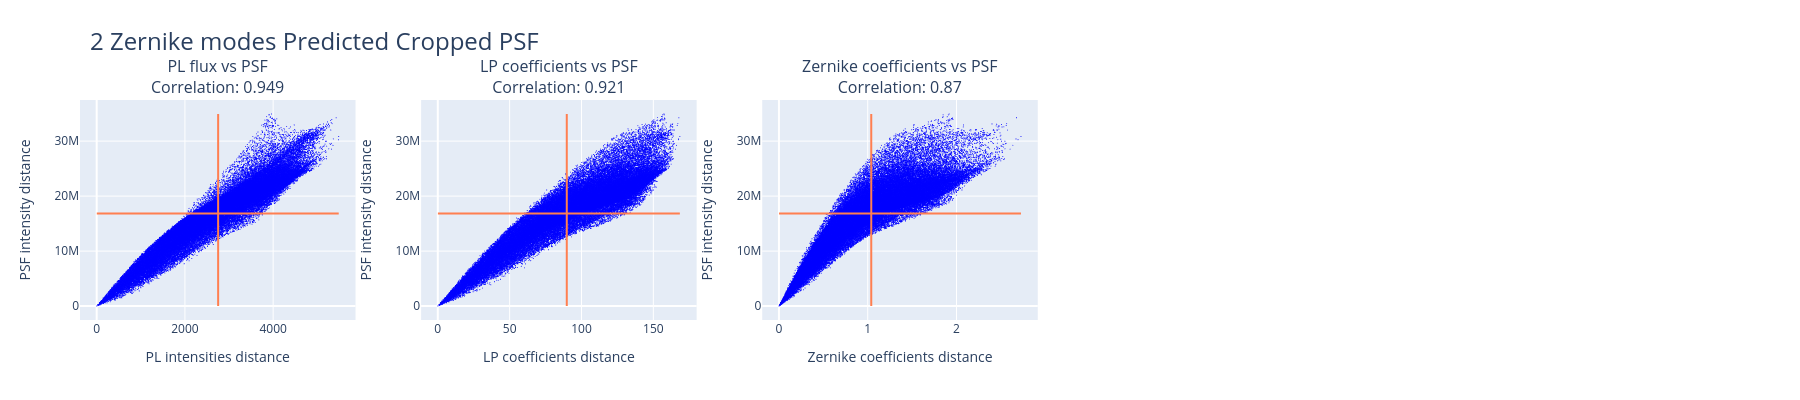
\includegraphics[width=0.7\textwidth]{pid-2mPredicted Croppedpsfdistances.png}}
			\\
			\subfloat[Euclidean distances for 5 zernike modes predicted cropped PSF intensity]{%
				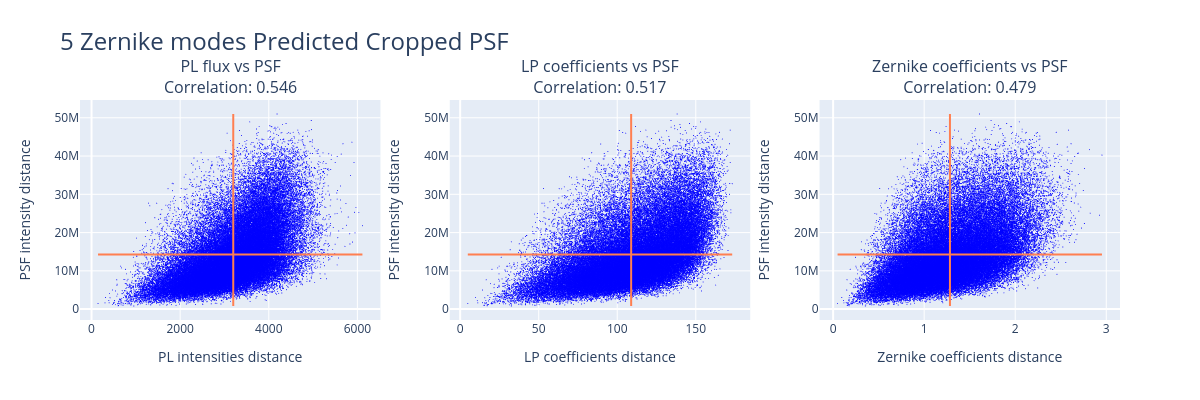
\includegraphics[width=0.7\textwidth]{pid-5mPredicted Croppedpsfdistances.png}}
			\\
			\subfloat[Euclidean distances for 9 zernike modes predicted cropped PSF intensity]{%
				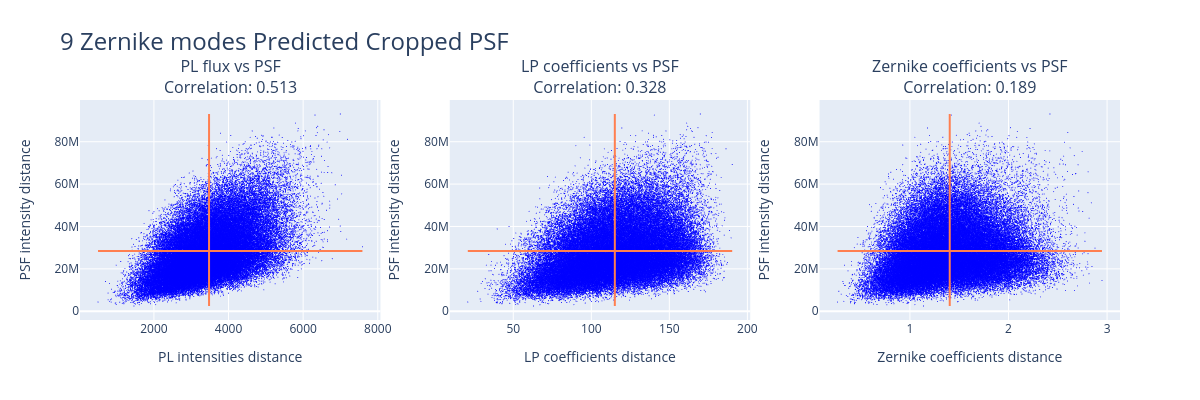
\includegraphics[width=0.7\textwidth]{pid-9mPredicted Croppedpsfdistances.png}}
			\\
			\subfloat[Euclidean distances for 14 zernike modes predicted cropped PSF intensity]{%
				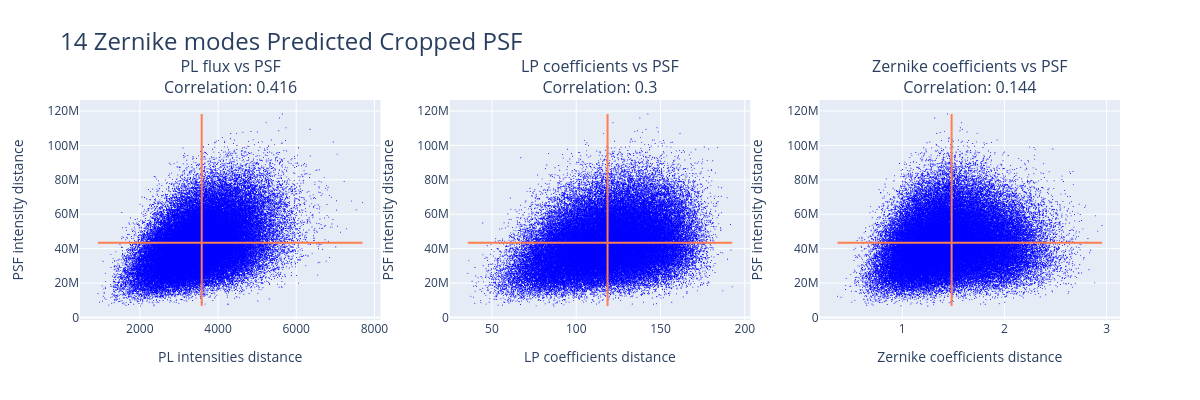
\includegraphics[width=0.7\textwidth]{pid-14mPredicted Croppedpsfdistances.png}}
			\\
			\subfloat[Euclidean distances for 20 zernike modes predicted cropped PSF intensity]{%
				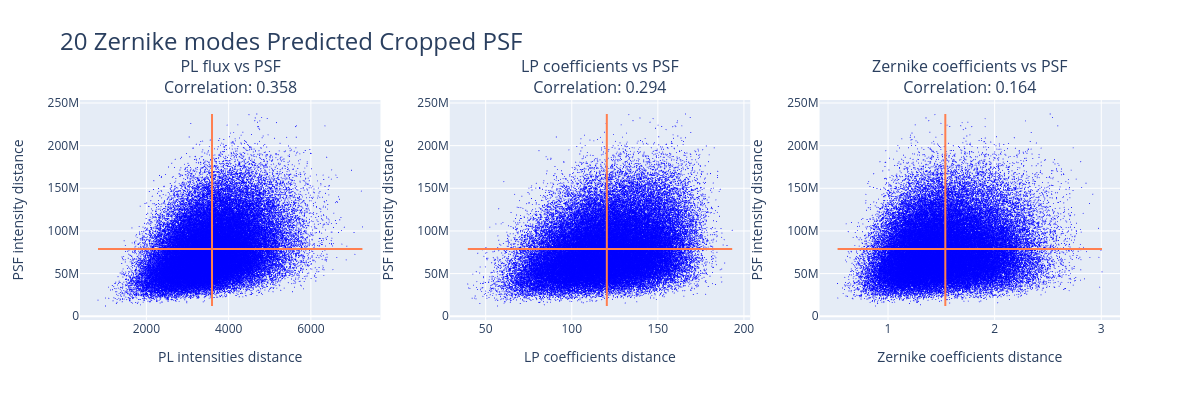
\includegraphics[width=0.7\textwidth]{pid-20mPredicted Croppedpsfdistances.png}}
				
			\caption{Euclidean distance comparison for predicted cropped PSF intensity for different number of modes}
		\end{figure*}
		\FloatBarrier
		
	\subsubsection{Analysis}
		\begin{itemize}
			\item The correlations between PSF distances and PL flux distances decay as the number of modes increases while the correlation between PSF distances and LP mode coefficients from the overlap integral are constant.
			\item The predicted psfs from the train datasets create a similar cloud of points to the original psfs which indicates that the models are capturing the information of the PL.
			\item The model trained for the dataset of 2 zernike terms PSF is the one that has the most overfit as the table shows (False, False, None indicate that no dropout, no batch normalization and no regularizer has been used), the validation mse just flatlines over the training.
			
			\item For 5 terms PSFs on the overfitting is reduced significantly although it increases with the number of zernike terms used. When using 20 terms the validation mse flatlines again.
			
			\item PL intensities vs PSF datasets evolution is practically the same for original, predicted, cropped and cropped predicted datasets. This indicates that the models are capturing accurately the relationship existing between the original PSF datasets and PL intensities datasets.
			
			\item LP coeffs vs PSF datasets evolution is practically the same for original, predicted, cropped and cropped predicted datasets.
		\end{itemize}
    
    
     
		\FloatBarrier